\section{Results}

\subsection{Framework Implementation and Performance}
% Addressing Objective 1: Present a systematic, AI-assisted framework for assembling and parameterizing EwE diet matrices

\subsubsection{Scale and Processing Efficiency}
We evaluated our framework through five independent runs across three distinct Australian regions, processing a total of 41,085 species. The framework handled 11,362 species in the Northern Territory's tropical reef ecosystem, 13,901 in the South East shelf's coastal and pelagic environments, and 15,822 in the South East Offshore's deep-water systems. 

\subsubsection{Computational Efficiency}
The computational requirements of the AI framework varied across regions. Total processing time ranged from 2.8 to 4.8 hours across regions. The most time-intensive stage was the downloading of biological data from online databases, accounting for approximately 70\% of the total processing time. Species identification typically required 0.01 hours, while the AI-driven species grouping process averaged 0.26 hours. Diet data collection and matrix construction required 0.7 and 0.04 hours respectively, with final parameter estimation taking 0.20 hours. On average, the framework required 0.7 seconds per species for data downloading and 0.2 seconds per species for diet data collection, though these rates varied considerably between regions due to differences in data availability and species complexity.
\begin{table}[htbp]
\centering
\footnotesize
\caption{Computational requirements by region and processing stage}
\label{tab:timing_analysis}
\begin{tabular}{lccccccc}
\hline
Region & Species & \multicolumn{6}{c}{Processing Time (hours)} \\
\cline{3-8}
 & Count & Identification & Data & Grouping & Diet & Matrix & Parameter \\
 & & & Download & & Collection & Construction & Estimation \\
\hline
v2 NorthernTerritory & 11,362 & 0.01 & 2.2 & 0.2 & 0.2 & 0.04 & 0.2 \\
v2 SouthEastInshore & 13,901 & 0.01 & 2.8 & 0.2 & 1.6 & 0.04 & 0.2 \\
v2 SouthEastOffshore & 15,821 & 0.01 & 3.3 & 0.4 & 0.3 & 0.04 & --- \\
\hline
\end{tabular}
\vspace{1ex}
\end{table}


Processing times varied by region and stage (Table \ref{tab:timing_analysis}). Data harvesting required 9.6 hours for the Northern Territory (3.0 seconds per species) and 53.8 hours for the South East shelf (13.9 seconds per species). Diet data collection took 7.6 hours for the Northern Territory (2.4 seconds per species) and 18.7 hours for the South East shelf (4.8 seconds per species). Species identification (0.01 hours), grouping (0.1 hours), and parameter estimation (0.1-0.3 hours) remained constant across regions.

\subsection{Species Grouping Validation}
% Addressing Objective 2a: Validate species grouping decisions and their ecological validity

\subsubsection{Classification Consistency and Ecological Validity}
The framework successfully reduced ecological complexity while preserving meaningful biological relationships. Starting with 63 potential functional groups provided in the default template (See Table \ref{tab:functional_groups}), it identified 34-37 region-specific groups, demonstrating its ability to capture unique ecological characteristics. Chi-square tests confirmed the ecological validity of these groupings, showing non-random species assignments across all regions (p < 0.001). This statistical significance provides strong evidence that the framework makes biologically informed grouping decisions rather than arbitrary assignments.

The precision of species assignments was assessed through coefficients of variation, which measure the relative variability in group assignments across iterations. These values revealed region-specific patterns: the Northern Territory showed moderate variation (1.47-15.20\%), reflecting the complexity of its tropical reef ecosystem. The South East shelf displayed the widest range (0.40-24.49\%), indicating greater flexibility in species assignments in this diverse coastal environment. The South East Offshore maintained intermediate variation (0.80-14.15\%), suggesting more stable classifications in its deep-water ecosystem.

To understand the significance of regional differences, we conducted ANOVA tests on group characteristics. The analysis revealed significant differences between regions, with effect sizes (Cohen's f) varying by metric type. Species-level metrics showed small effect sizes (0.1-0.3), indicating subtle but consistent regional variations in how individual species were classified. Group-level comparisons showed large effect sizes (>0.4), demonstrating that the framework successfully captured distinct regional ecological structures.

The framework achieved remarkable classification stability across all regions. Mean consistency scores, where 1.0 represents perfect stability, were exceptionally high: 0.997 for both Northern Territory and South East shelf, and 0.998 for South East Offshore. This translated to very low proportions of unstable species (defined as consistency < 0.95): only 0.99\% (103 species) in Northern Territory, 1.06\% (125 species) in South East shelf, and 0.73\% (87 species) in South East Offshore. These results demonstrate that the framework's classifications remained stable despite the stochastic nature of the AI decision-making process.

Figure \ref{fig:regional_analysis} presents the quantitative analysis across regions. Panel A shows median group sizes of 150-200 species, indicating consistent ecological partitioning across regions. Panel B displays consistency scores, revealing that while the Northern Territory showed some variation (0.4-1.0), the South East regions maintained higher minimum consistency (0.8-1.0). Panel C demonstrates the framework's stability through Jaccard similarity indices, which measure group membership consistency between iterations. The Northern Territory achieved similarities of 0.953-0.999, indicating high stability with some flexibility in species assignments. South East shelf ranged from 0.867-1.000, and South East Offshore from 0.855-1.000, both showing perfect stability in some groups while allowing ecological adaptability in others. Panel D quantifies this variation, showing tighter control in South East regions (5-10 species standard deviation) compared to the more dynamic Northern Territory system (15-35 species).

The stability heatmap (Figure \ref{fig:stability_heatmap}) reveals patterns in group stability that reflect ecological principles. In the Northern Territory, benthic groups showed highest stability (benthic infaunal carnivores: 0.999, benthic filter feeders: 0.992, benthic grazers: 0.989), while more mobile groups showed greater variation (deposit feeders: 0.953, planktivores: 0.956). The South East shelf achieved perfect stability for macrozoobenthos (1.000) but showed more variation in pelagic groups (piscivores: 0.867, oceanic piscivorous fish: 0.897), reflecting the dynamic nature of its coastal environment. South East Offshore demonstrated perfect stability in benthic filter feeders (1.000) but greater variation in planktonic groups (nanoplankton: 0.855) and piscivores (0.941).

\begin{figure}[htbp]
    \centering
    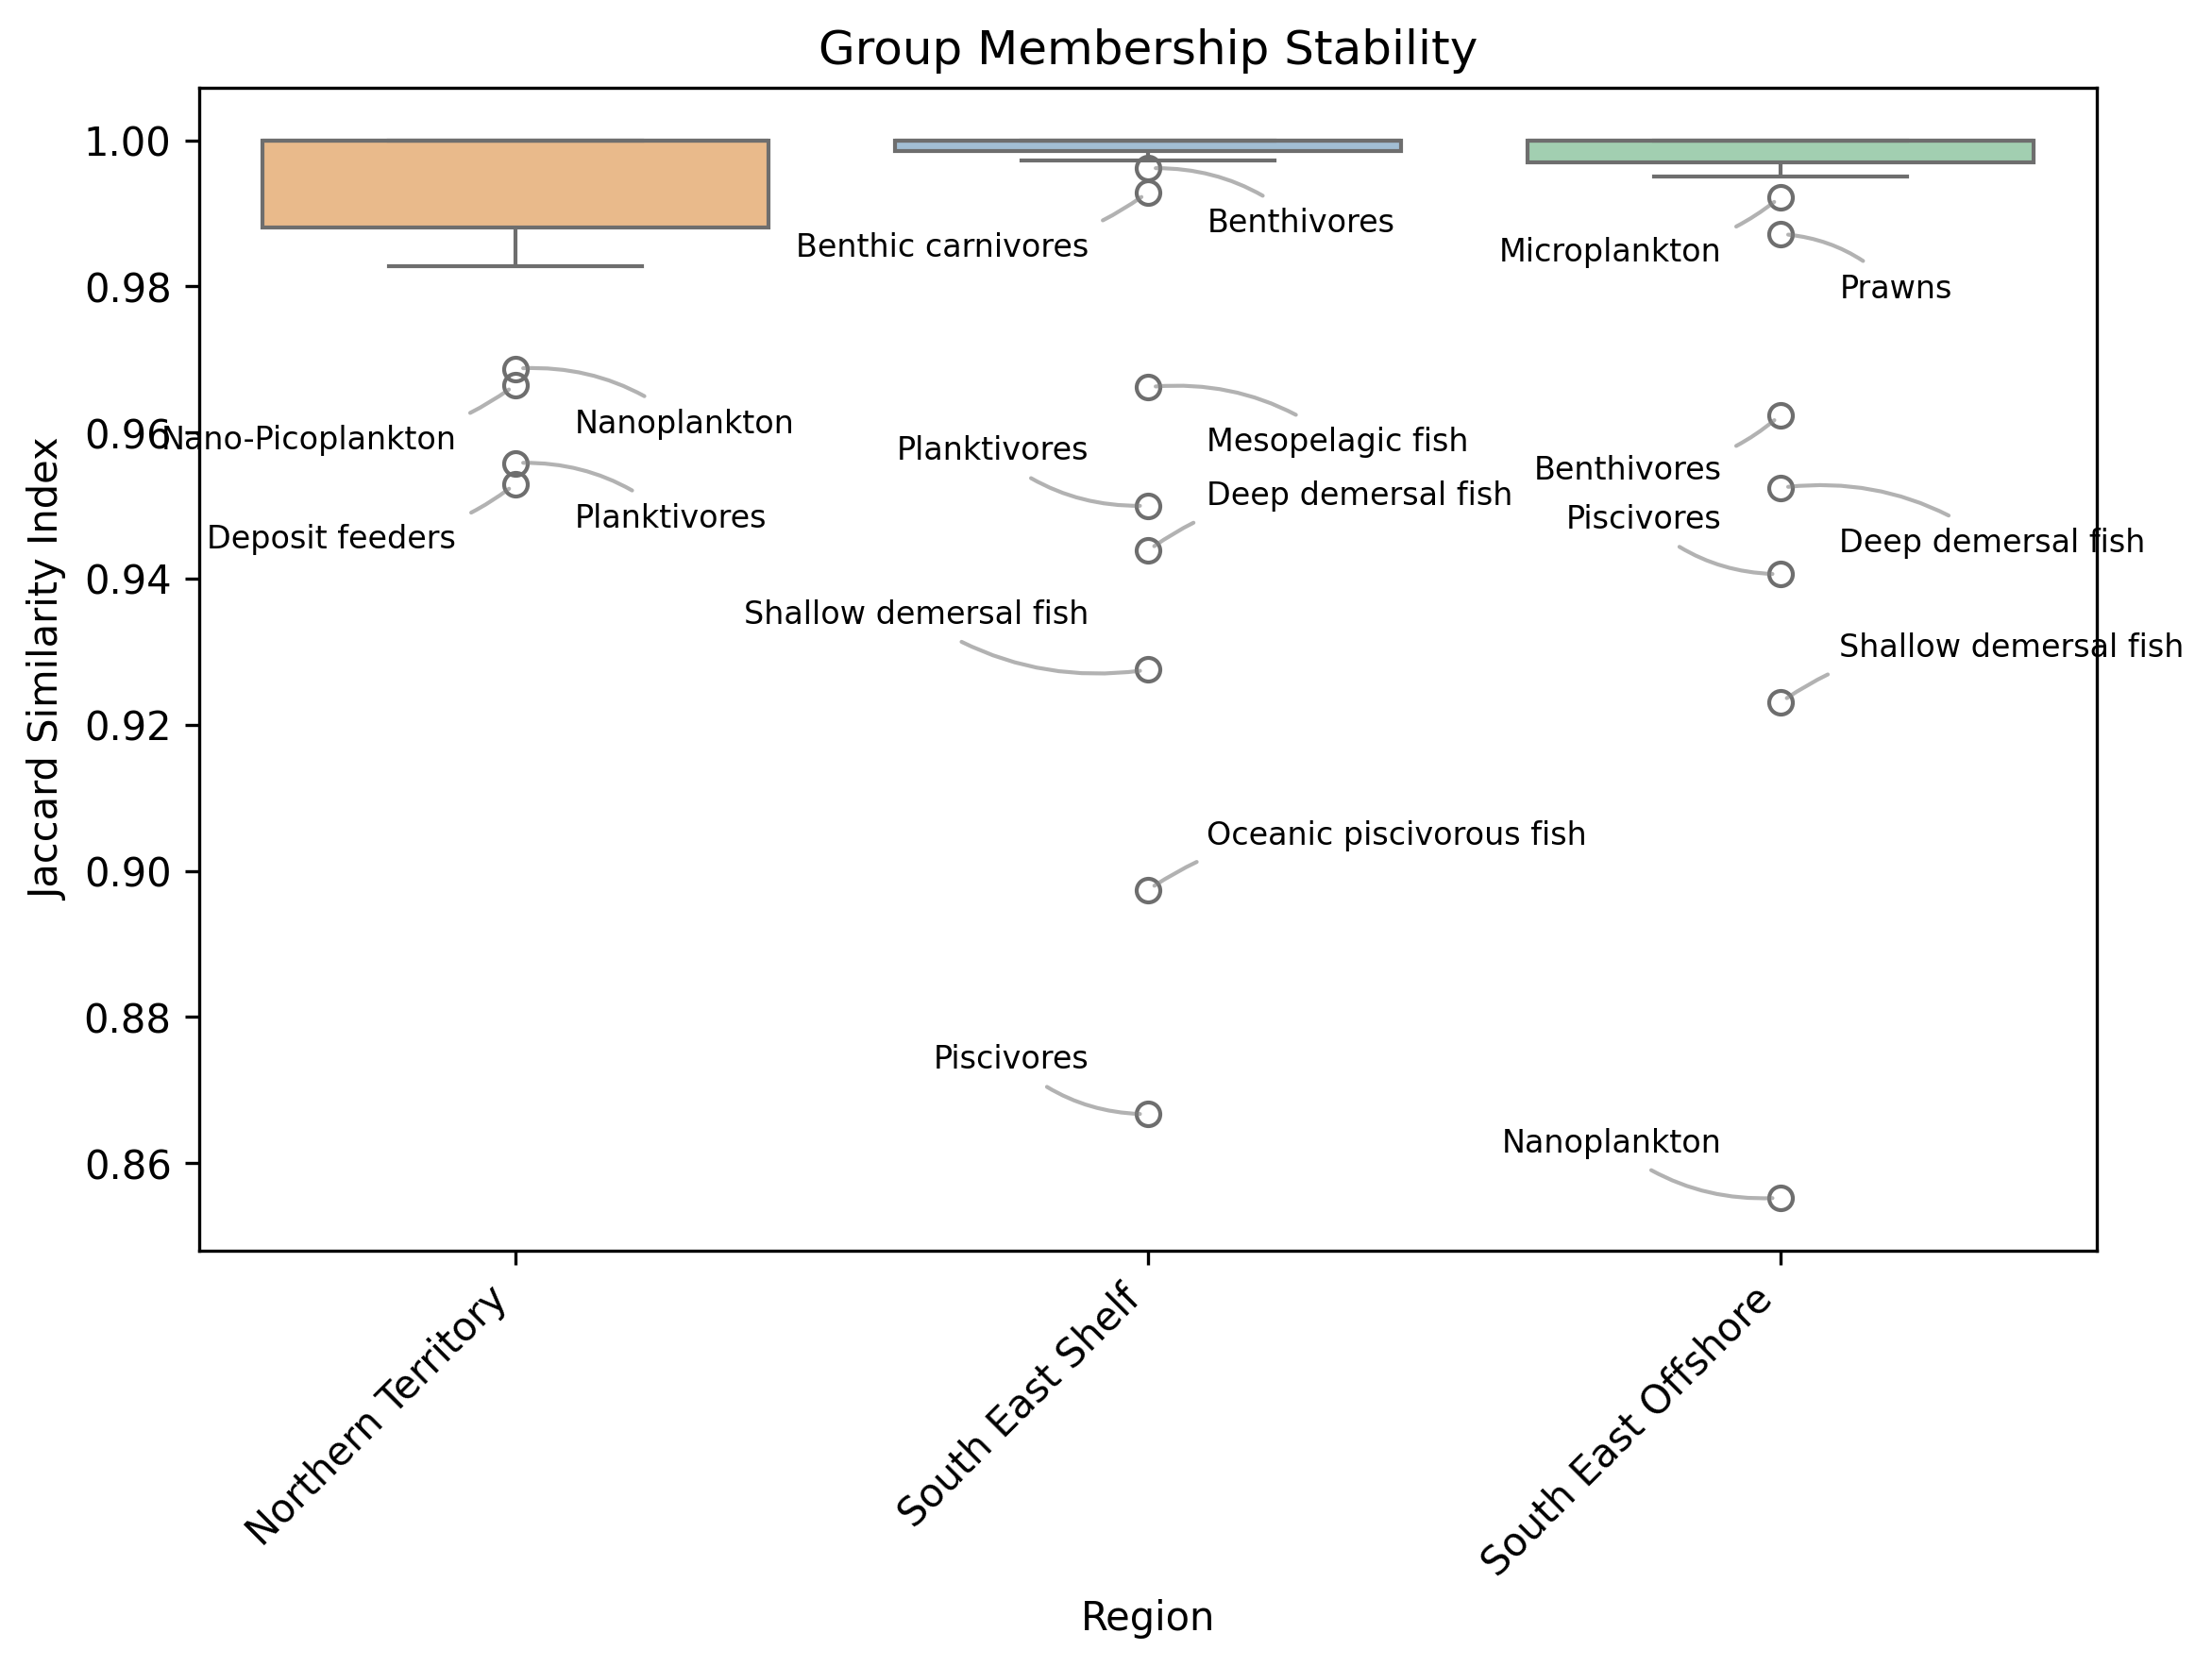
\includegraphics[width=\textwidth]{figures/regional_group_analysis.png}
    \caption{Multi-panel analysis of framework performance across regions. (A) Box plots of functional group sizes (0-3000 species), showing similar median sizes but varying distributions across regions, with outliers indicating some very large groups. (B) Violin plots of species classification consistency (0.4-1.0), where wider sections indicate more species with that consistency score; most species show high consistency (>0.9) with slightly more variation in the Northern Territory. (C) Box plots of group stability measured by Jaccard similarity (0.975-1.000), showing highest stability in South East Offshore and more variable stability in Northern Territory. (D) Box plots of group size variation (standard deviation 0-35), demonstrating larger fluctuations in group membership in the Northern Territory compared to South East regions.}
    \label{fig:regional_analysis}
\end{figure}

\begin{figure}[htbp]
    \centering
    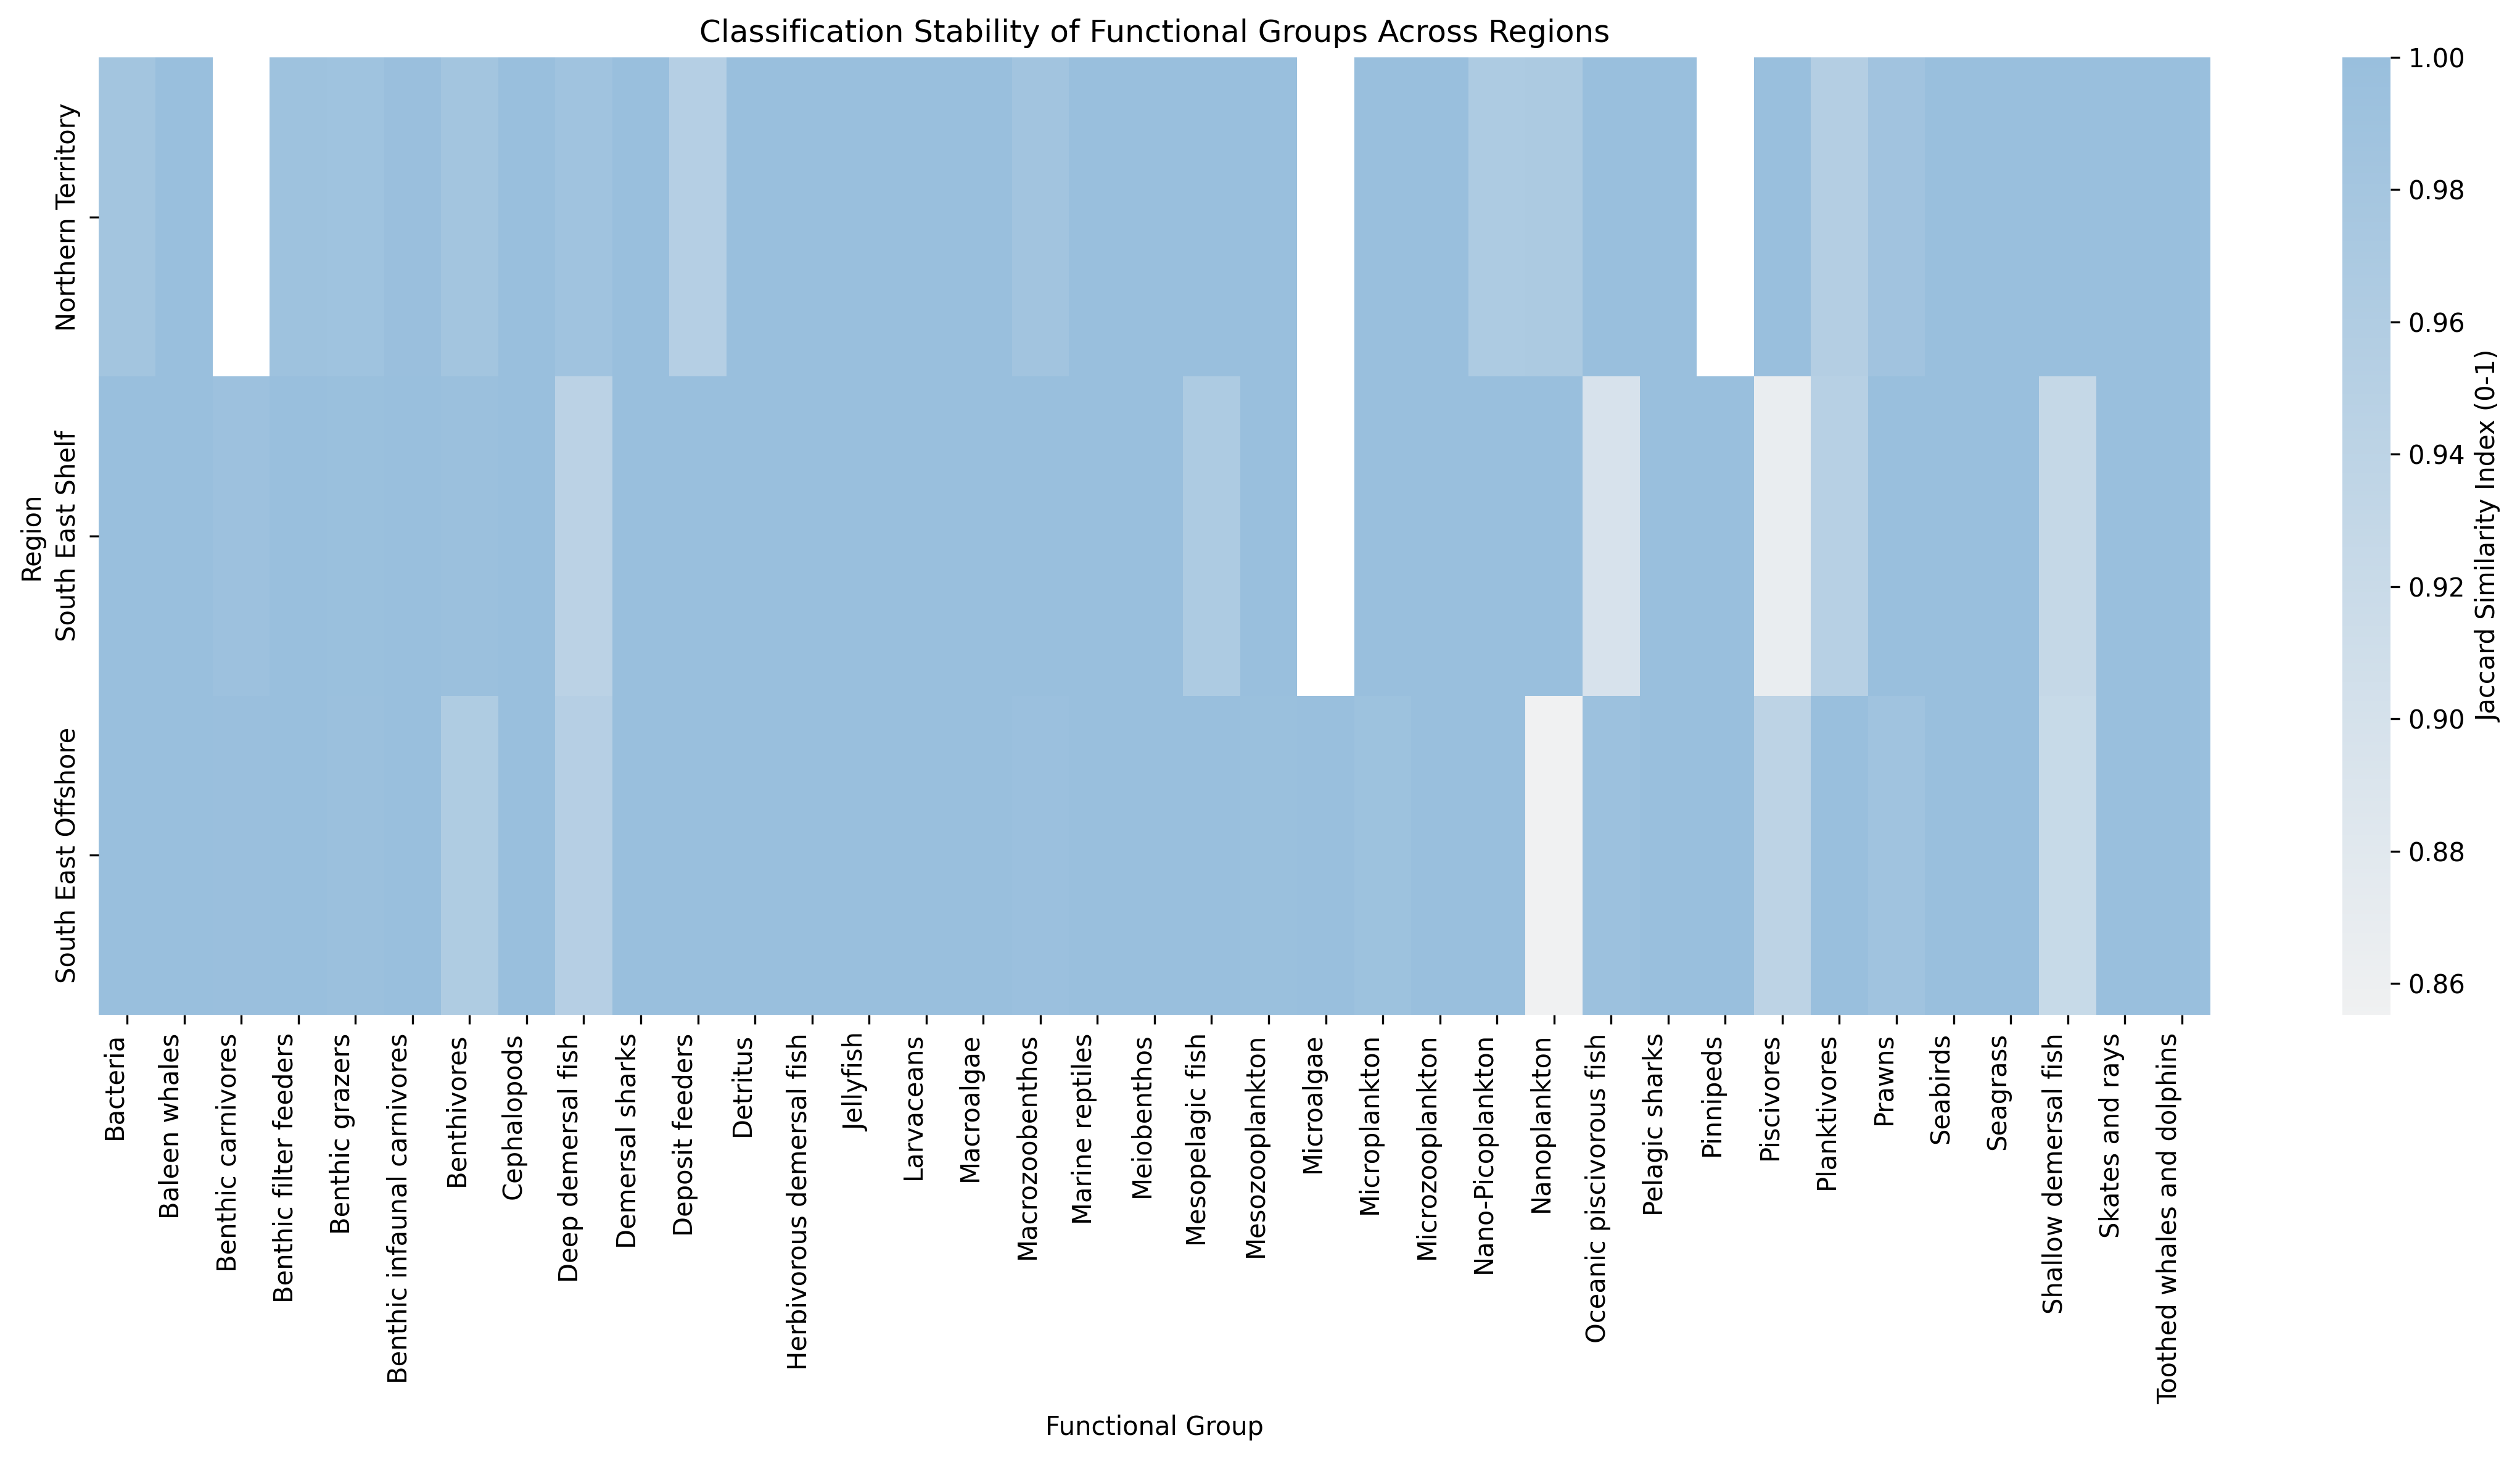
\includegraphics[width=\textwidth]{figures/group_stability_heatmap.png}
    \caption{Heatmap showing the stability of functional group classifications across regions. Each cell displays the Jaccard similarity score (ranging from 0.975 to 1.000) between consecutive framework iterations, where 1.000 indicates perfect consistency in species assignments. Darker red colors represent higher stability (scores near 1.000), while lighter colors indicate more variable classifications (scores closer to 0.975). Most functional groups show high stability (>0.99) across all regions, with occasional variations in groups like benthic grazers and deposit feeders, particularly in the Northern Territory region.}
    \label{fig:stability_heatmap}
\end{figure}

\begin{table}[htbp]
\centering
\caption{Dominant patterns of species classification instability across three study regions. The table presents the most frequent oscillation patterns between functional groups for species that were inconsistently classified across the five framework iterations. For each region, the total number of variably classified species is shown (representing less than 1.1\% of all species), along with the percentage distribution of different oscillation patterns.}
\label{tab:unstable_species}
\small
\begin{tabular}{llcc}
\hline
Region & Most Common Pattern & Count & \% of Total \\
\hline
Northern & Macrozoobenthos $\leftrightarrow$ Benthic infaunal carnivores & 28 & 27.2\% \\
Territory & Benthic filter feeders $\leftrightarrow$ Deposit feeders & 25 & 24.3\% \\
(103 species) & Prawns $\leftrightarrow$ Macrozoobenthos & 21 & 20.4\% \\
& Other patterns & 29 & 28.1\% \\
\hline
South East & Piscivores $\leftrightarrow$ Deep demersal fish & 42 & 33.6\% \\
Inshore & Benthic grazers $\leftrightarrow$ Benthic carnivores & 31 & 24.8\% \\
(125 species) & Planktivores $\leftrightarrow$ Mesopelagic fish & 28 & 22.4\% \\
& Other patterns & 24 & 19.2\% \\
\hline
South East & Benthic filter feeders $\leftrightarrow$ Benthic carnivores & 25 & 28.7\% \\
Offshore & Macrozoobenthos $\leftrightarrow$ Deep demersal fish & 22 & 25.3\% \\
(87 species) & Mesozooplankton $\leftrightarrow$ Macrozoobenthos & 18 & 20.7\% \\
& Other patterns & 22 & 25.3\% \\
\hline
\multicolumn{4}{p{0.95\textwidth}}{\small \textit{Note:} Arrows indicate group assignment oscillation between iterations. Complete species-level data available in Section S3 of the supplementary material.} \\
\hline
\end{tabular}
\end{table}


\subsection{Diet Matrix Consistency}
% Addressing Objective 2b: Validate diet matrix values and their reliability

\subsubsection{Trophic Interaction Stability}
The framework demonstrated consistent performance in constructing diet matrices, with consistency patterns aligning with known ecological principles. Our stability score metric (0 = perfect stability, 1 = maximum variation) revealed region-specific patterns in trophic relationship consistency:

\begin{itemize}
    \item Northern Territory: 358 significant predator-prey interactions identified, with 58.7\% achieving high stability (scores < 0.3), reflecting expected variability in complex tropical reef food webs
    \item South East shelf: 380 interactions with 51.3\% stable, indicating characteristic trophic plasticity in dynamic coastal environments
    \item South East Offshore: 477 interactions with 56.0\% stable, suggesting more consistent feeding relationships typical of deep-water ecosystems
\end{itemize}

To validate these patterns, we calculated Spearman correlations between iterations for significant interactions, providing a measure of consistency in diet proportion rankings. All regions showed strong correlations: Northern Territory ($\rho = 0.72-0.89$), South East shelf ($\rho = 0.68-0.85$), and South East Offshore ($\rho = 0.70-0.87$). These high correlations indicate that while absolute diet proportions might vary, the relative importance of different prey items remained consistent across iterations.

\begin{figure}[htbp]
    \centering
    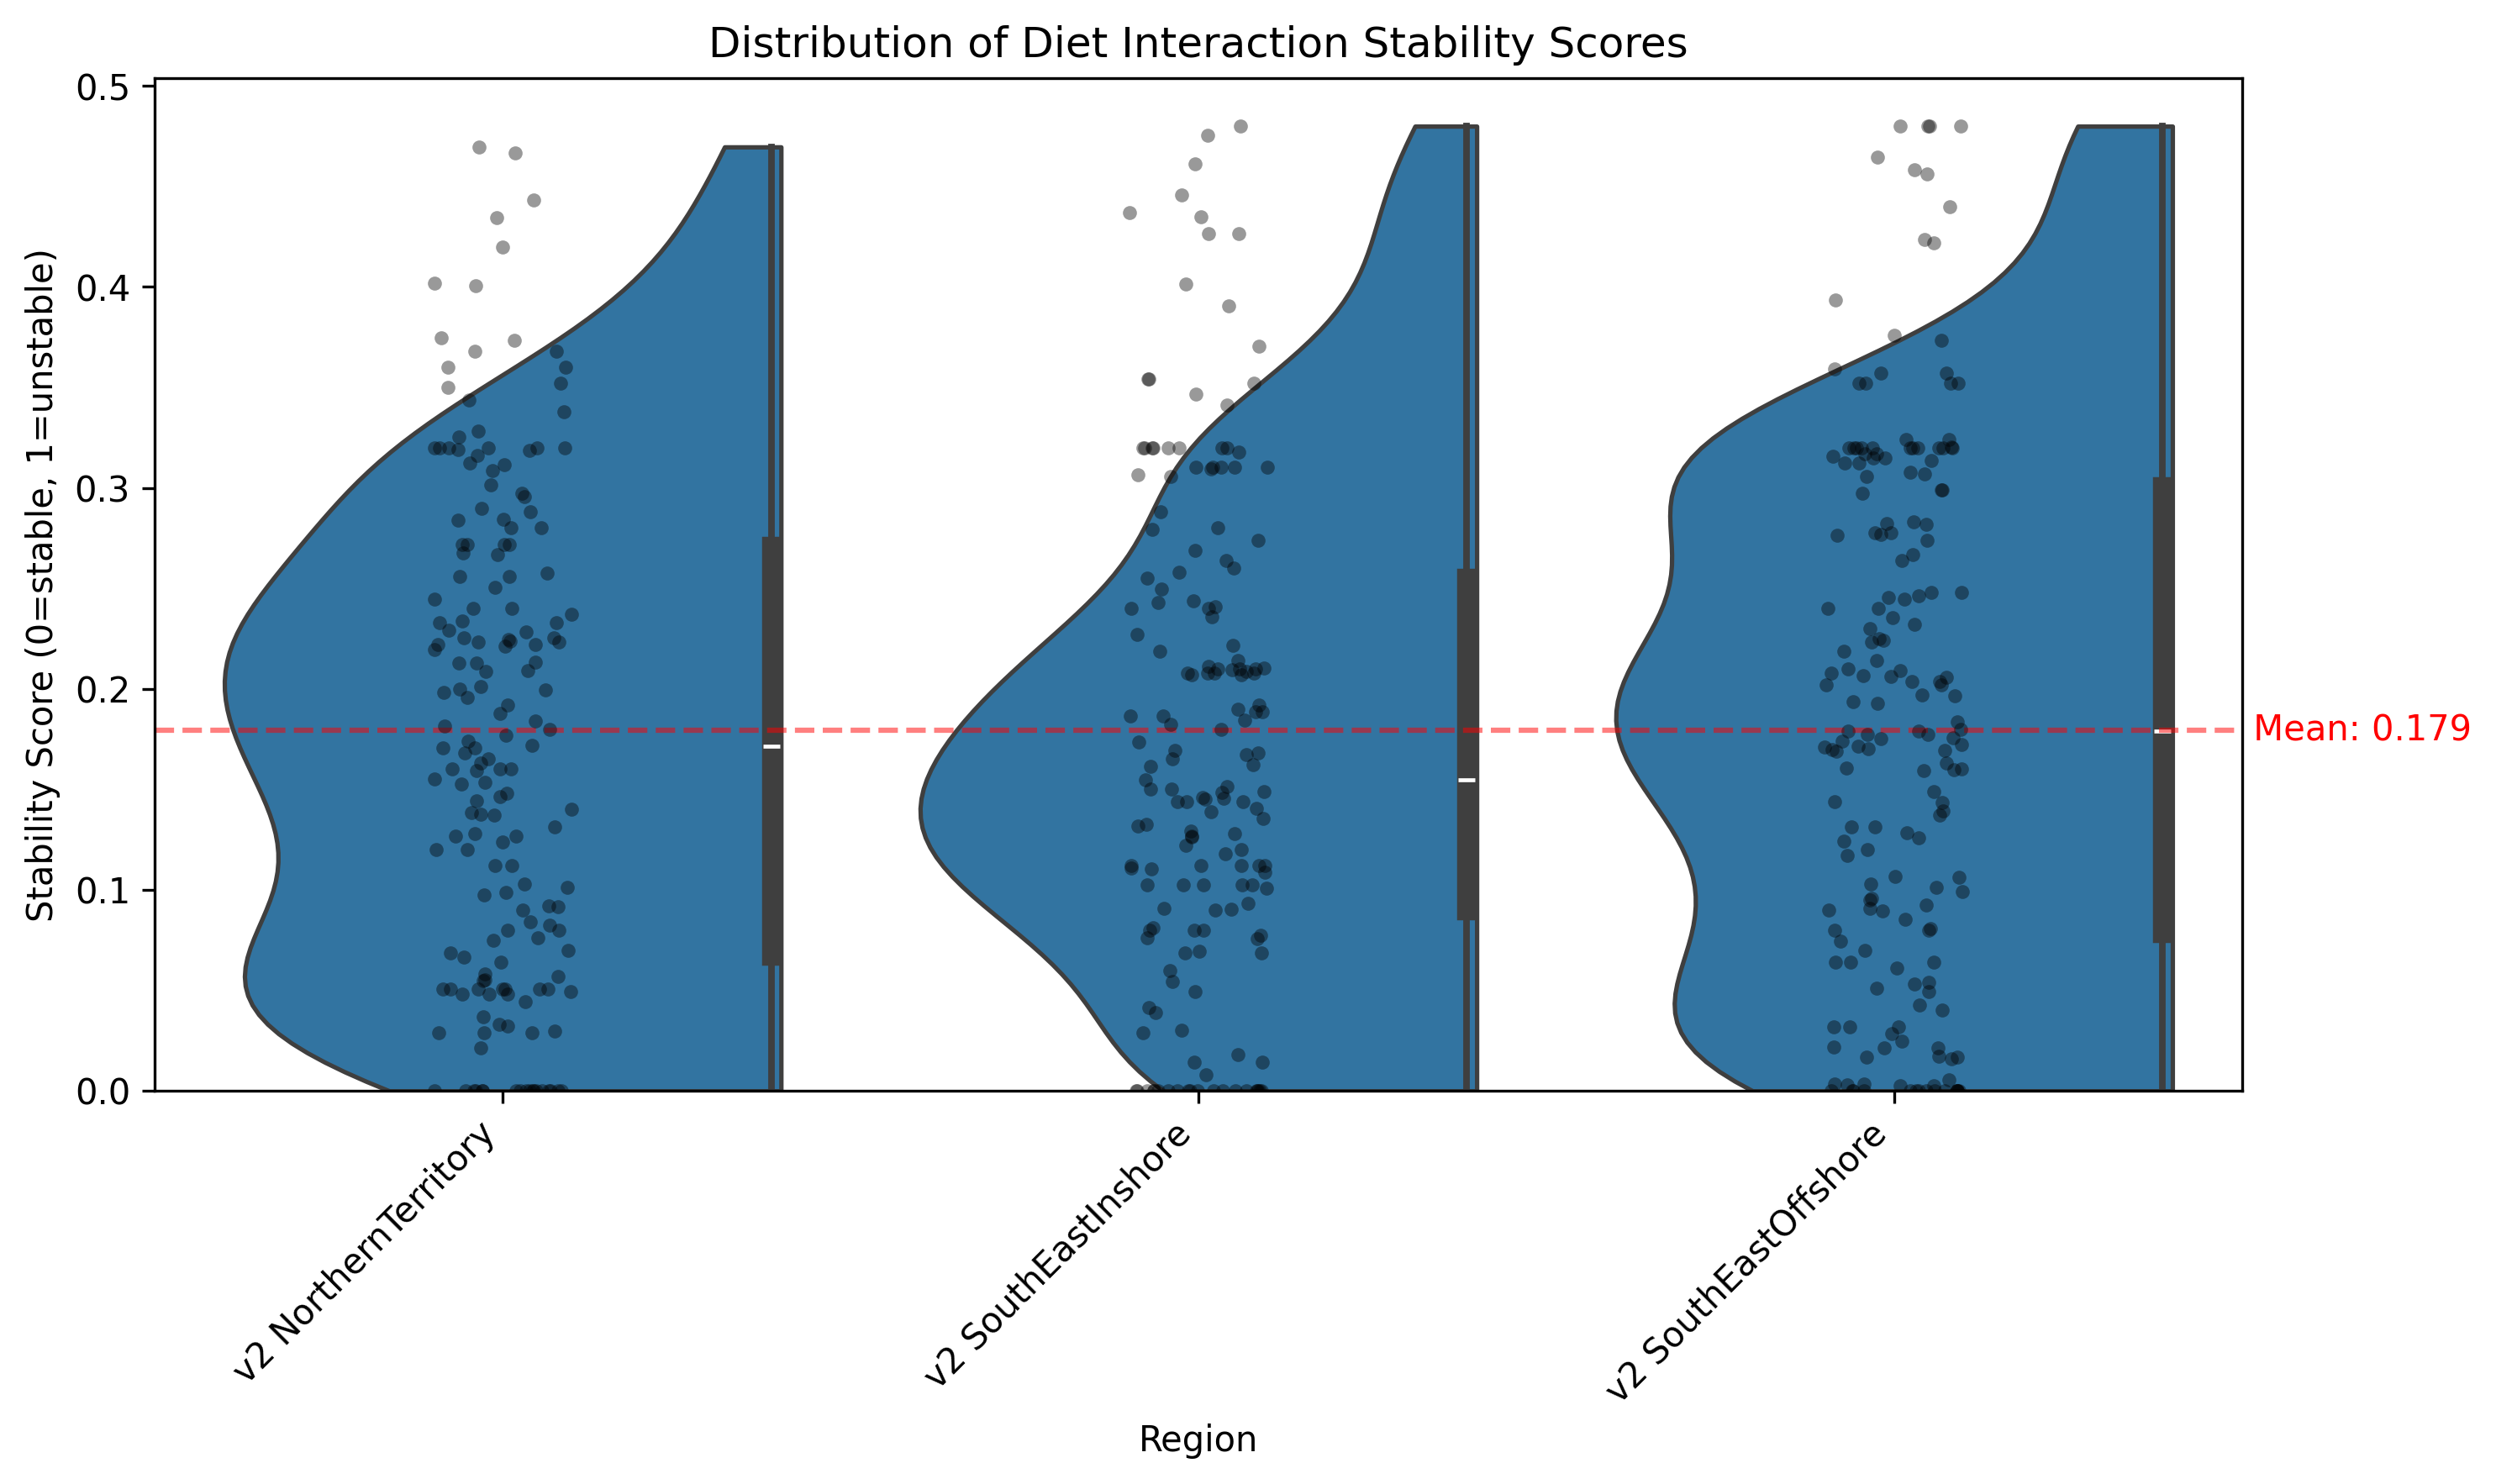
\includegraphics[width=\textwidth]{figures/stability_score_distribution.png}
    \caption{Distribution of diet interaction stability scores across regions. Half-violin plots show the density of stability scores (0=stable, 1=unstable), with embedded box plots indicating quartiles and median. Individual points represent specific predator-prey interactions, and the red dashed line shows the mean stability score across all regions. The distributions are bounded at zero, reflecting perfect stability, with most interactions showing scores below 0.3.}
    \label{fig:stability_distribution}
\end{figure}

Analysis of stability scores by predator group revealed ecological patterns consistent with trophic theory. The most stable interactions were found in detritus-based and primary producer connections, reflecting the fundamental nature of these energy pathways in marine ecosystems. Predator-prey relationships in higher trophic levels showed more variation, consistent with the opportunistic feeding strategies of marine predators. Benthic feeding relationships demonstrated intermediate stability, suggesting a balance between dietary specialization and opportunism in these communities. These patterns align with ecological understanding that diet variability typically increases with trophic level, reflecting the more generalist feeding strategies of higher-level predators. Detailed diet matrices for each region are provided in the supplementary material (Figure~S1).

\begin{figure}[htbp]
    \centering
    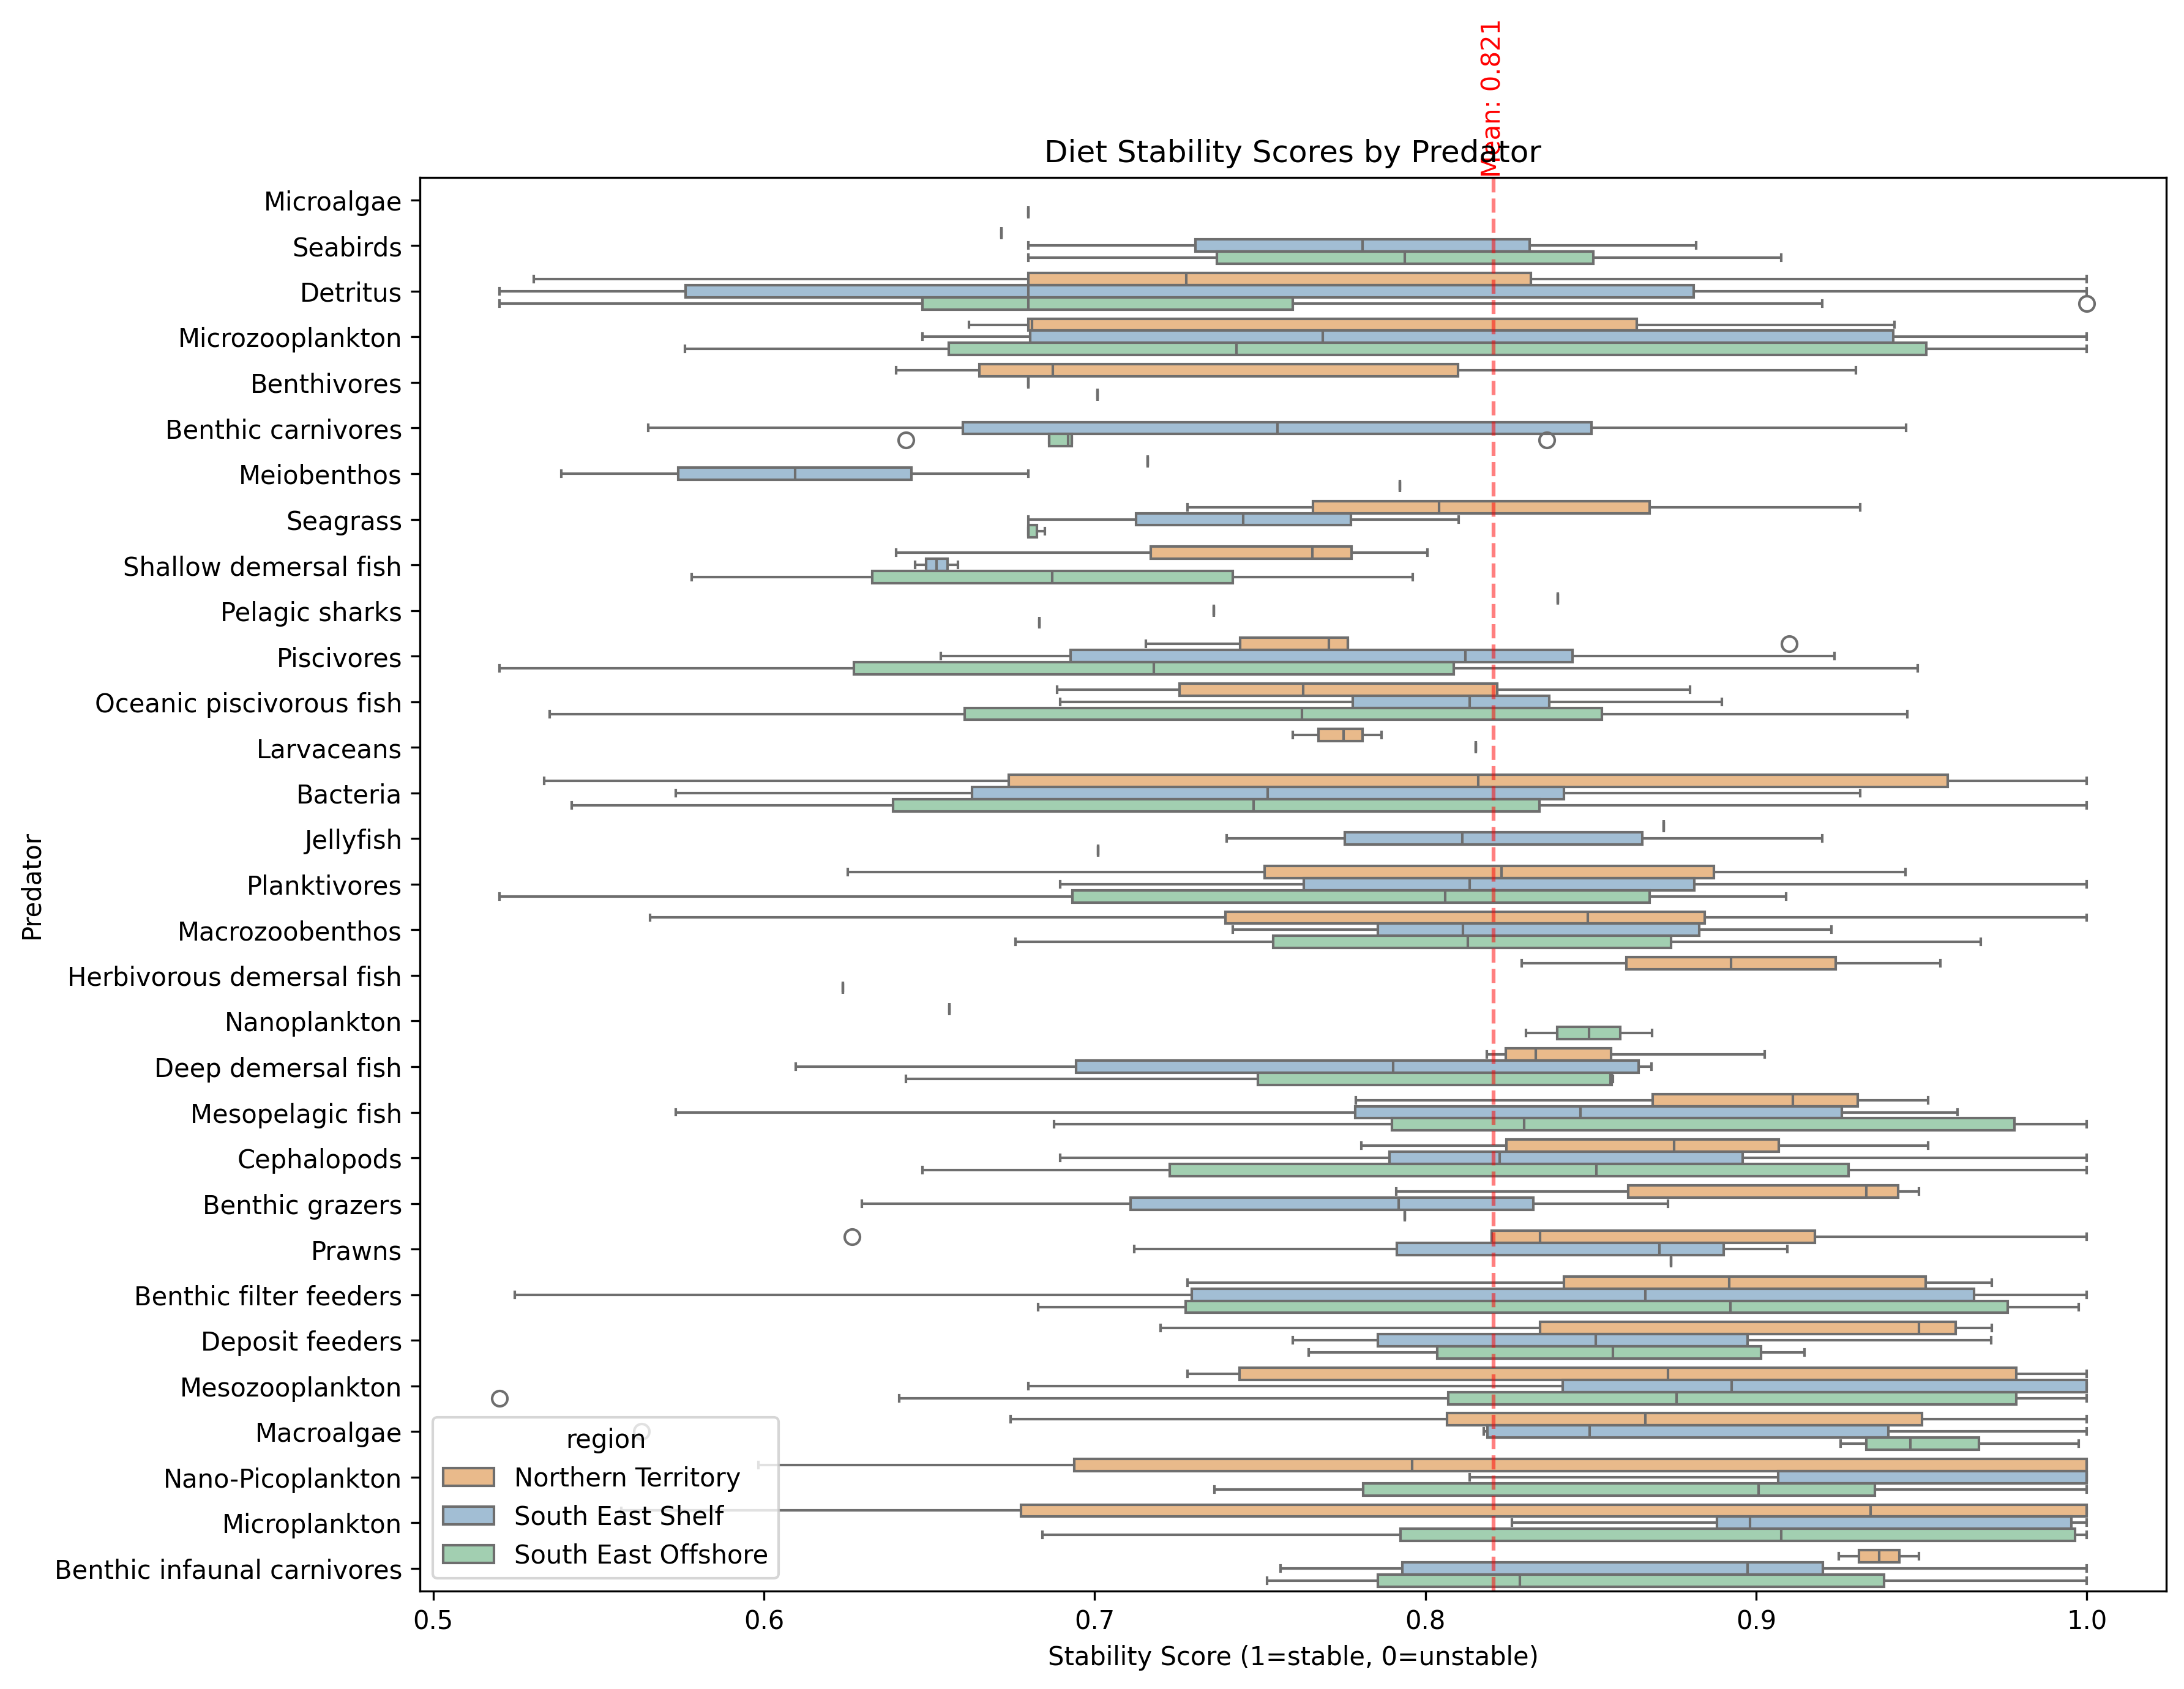
\includegraphics[width=\textwidth]{figures/predator_stability_boxplots.png}
    \caption{Diet stability scores grouped by predator, ordered by median stability. Box plots show the distribution of stability scores for each predator's diet across regions (colored by region). The red dashed line indicates the mean stability score across all predator-prey interactions. Lower scores indicate more consistent diet compositions across framework iterations.}
    \label{fig:predator_stability}
\end{figure}

\subsection{Regional Adaptability}
% Addressing Objective 3: Assess framework's applicability across different marine ecosystems

\subsubsection{Ecosystem-Specific Performance}
The framework demonstrated significant capability to adapt to distinct marine ecosystems while maintaining ecological validity. Trophic structure analysis revealed statistically significant regional differences (Kruskal-Wallis H-test: Northern Territory H = 164.0, South East shelf H = 172.0, p < 0.001 for both), confirming the framework's ability to capture unique ecosystem characteristics. Key findings include:

\begin{itemize}
    \item Higher trophic levels: Consistent classifications across regions for apex predators and specialized feeders, demonstrating robust handling of well-defined ecological roles
    \item Lower trophic levels: Greater variability in planktonic and benthic invertebrate groups, reflecting natural ecological plasticity
    \item Mid-trophic levels: Moderate variation in species assignments (e.g., benthivores: 715-788 species, shallow demersal fish: 586-659 species), aligning with expected ecological flexibility in these groups
\end{itemize}

These patterns demonstrate the framework's ability to balance consistency with necessary ecological flexibility across different marine environments.
